Section consists mainly of bullet-points
\section{General considerations}
\subsection{Desirable attributes}
\begin{itemize}
\item \textbf{Suitability for application}.
\item \textbf{Cost of use}. There are many relevant costs to take into account. They include
\begin{itemize}
\item cost of program execution
\item cost of compilation
\item cost of program creation and testing
\item cost of maintenance
\end{itemize}
\item \textbf{Programming environment}. Existence of external tools to ease development.
\item \textbf{Portability}.

\item \textbf{Readability} and, usually to a lesser extent, \textbf{writability}. Much more time is spent reading code than writing code, so optimise for readability, not terseness or compactness.

\item \textbf{Conceptual clarity, simplicity and unity}. Different concepts and constructs should fit together understandably. This is called \emph{conceptual integrity}.

This also means there should be no ambiguity.

\item \textbf{Promoting understandable programs}. This point is related to the last two. Ideally the language should promote the use of conceptually clear solutions.

\item \textbf{Orthogonality}. As many different attributes of the language should fit together as possible. Downsides of orthogonality include allowing inefficient constructs and more difficult program verification.

\item \textbf{Support for abstraction}.
\item \textbf{Ease of program verification}. Techniques for program verification include
\begin{itemize}
\item formal verification methods (proofs of correctness)
\item desk checking (i.e. visual inspection)
\item testing.
\end{itemize}
\item \textbf{Context free grammar}. 
\end{itemize}

\subsection{Operating environments}
Programming languages can be designed to work in different operating environments. The target environment has profound implications for the design of the language.
\begin{itemize}
\item Interactive environments (usually with a graphical user interface).
\item Batch-processing environments where input (usually in the form of files) is given and the program computes the output.
\item Embedded system environments.
\end{itemize}

\subsection{Thoughts on optimizing information transmission}
\begin{itemize}
\item It is easier to master static relations, than visualize processes evolving in time. We should shorten the conceptual gap between the static program (in text space) and the dynamic process (spread out in time). (Dijkstra)
\end{itemize}

\section{Language paradigms}
Language paradigms refer to the conceptual ideas that dictate the language's feature set. There are many different (mostly not mutually exclusive) programming paradigms. A language can support multiple paradigms.

The biggest distinction is between \udef{imperative} and \udef{declarative} languages. 
\begin{itemize}
\item Imperative languages tell the computer \textit{how} to perform calculations. Programs in imperative languages are typically a list of statements. Machine languages are imperative, so all computer languages eventually get translated into an imperative form. An imperative language may support the following paradigms:
\begin{itemize}
\item \textbf{Procedural}, which groups instructions into procedures (also called subroutines).
\item \textbf{Object-oriented},  which groups instructions together with the data they operate on.
\end{itemize}
\item Declarative languages declare the properties of the desired result but not how to compute it. Declarative paradigms include:
\begin{itemize}
\item \textbf{Functional}, in which the desired result is declared as the value of a series of function applications.
\item \textbf{Logic programming}, in which the desired result is inferred from logical statements.
\end{itemize}
\end{itemize}

Several paradigms will be discussed in more depth when discussing concrete languages.

\section{Some common language features}
These are some common features shared by many languages. The information here is intentionally quite vague, as every language implements these features in different ways. The ideas presented here will be made much more concrete when looking at specific languages. Any particular language may only support some of these features.
\begin{itemize}
\item \textbf{Statements} are the basic building blocks of imperative languages. They instruct the computer which action to carry out next.
\item \textbf{Data types} define how raw binary data should be interpreted. Examples include:
\begin{itemize}
\item \textbf{Integers} are (positive or negative) whole numbers. Many programming languages can only represent numbers up to a certain size.
\item \textbf{Floats} are floating point numbers, i.e. real numbers. Many programming languages can only represent numbers up to a certain size and precision.
\item \textbf{Arrays} are lists of values.
\item \textbf{Pointers} refer to specific locations in memory.
\end{itemize}
\item \textbf{Literals} are concrete representations of data that the computer can readily convert to a binary representation. Examples include numeric literals (such as $42$ or $22.45$), boolean literals (such as \textit{true} and \textit{false}), string literals (such as ``Hello world'') and array literals (such as $[1,2,5,6]$).
\item \textbf{Expressions} generally produce a value of a certain type. They may be literals, or a description of which operations to carry out in order to get the required value.
\item \textbf{Variables} are named locations we can use to store values (usually of a particular type).
\item \textbf{Control structures} control which statements get executed in which order.
\begin{itemize}
\item \textbf{Conditionals} evaluate an expression. Depending on the result, the program does different things. The two most common constructs are
\begin{itemize}
\item \undline{if-then-else} statements (which execute the then part only if the expression evaluates to true) and
\item \undline{case-and-switch} statements (which evaluate an expression and choose the correct course of action by comparing the value to several different case statements).
\end{itemize}
\item \textbf{Loops} execute a block of code multiple times.
\begin{itemize}
\item \undline{While loops} checks a condition every loop and while that condition is true it keeps on looping.
\item \undline{For loops} generally do a loop for each value in a given set.
\item A language may also provide \undline{break} and \undline{continue} statements in order to, respectively, immediately break out of a loop and move on to the next iteration of the loop.
\end{itemize}
\item \textbf{Subroutines} are sequences of program instructions that each perform a specific task, packaged as a unit. This unit can then be used in programs wherever that particular task should be performed. Often subroutines require arguments to operate on. A subroutine may also be called a \textbf{procedure}, a \textbf{function}, a \textbf{routine} or a \textbf{subprogram}, depending on the language. If the subroutine is bundled with data (such as in the object-oriented paradigm), it is conventionally called a \textbf{method}.
\item \textbf{Coroutines} are functions that can yield control to each other.
\item \textbf{Generators}, also known as \textit{semicoroutines}, are functions that are in fact iterators, i.e. at each call it returns the next value in a sequence.
\item The \textbf{goto} statement causes the next statement to be executed to be the one at a particular \textbf{label}. Goto statements have been considered harmful by many programmers. The main points of the discussion are summarized in a later section.
\item \textbf{Exceptions} are \textit{thrown} during anomalous or exceptional conditions. Hopefully there is then code that can \textit{catch} the exception and handle accordingly. The exact notion of exceptions differs between languages. In some it is supposed to be used solely to handle abnormal, unpredictable or erroneous situations. In some it may be used for flow control structures. 
\end{itemize}
\item Some features typical for object oriented programming include:
\begin{itemize}
\item \textbf{Objects} are usually containers with named fields containing data of different types as well as subroutines acting on the object (called methods).
\item \textbf{Classes} can specify what type of data objects contain as well as which methods they have. They can be seen as a way to define custom types.
\item New classes can be built based on old classes. This is called \textbf{inheritance}.
\end{itemize}
\item \textbf{Regular expressions} are used to match (parts of) text, as discussed above.
\end{itemize}

\section{Syntactic elements of a language}
\begin{itemize}
\item \textbf{Character set}. Which encoding is to be used?
\item \textbf{Identifiers} are names for things like variables and subroutines. Typically they are subject to some restrictions, like not being able to start with a number, or not being a reserved words.
\item \textbf{Keywords} and \textbf{reserved words} are words that may not be used as identifiers, typically because they have some special meaning in the language.
\item \textbf{Operator symbols}
\item \textbf{Comments} consist of text in the program that is ignored during execution. The purpose of comments is to explain what the program is doing.
\item \textbf{Blanks} are usually used to separate other syntactic elements. Sometimes they have other uses, such as newlines terminating statements in Python.
\item \textbf{Delimiters} and \textbf{brackets}.
\end{itemize}
Here we may also remark upon the benefits of the (judicious) use of \udef{syntactic sugar}. These are syntactic constructs that do not add any real functionality to the language, but merely provide an easier syntax for commonly used constructs.

This term has spawned some related concepts:
\begin{itemize}
\item \udef{Syntactic salt} refers to a language feature designed to make it harder to write bad or incorrect code.
\item \udef{Syntactic saccharin} or \udef{syntactic syrup} refers to gratuitous syntax that does not make programming any easier.
\end{itemize}

\section{Practical aspects of data types}
This is a more practical overview of some aspects of data types .
\subsection{Data type specification}
The basic elements of a specification of a data type are:
\begin{enumerate}
\item The possible \textbf{values} that data objects of that type may have.
\item The \textbf{attributes} that distinguish data objects of that type. Some of the attributes may be stored in a \udef{descriptor} (also called a \udef{dope vector}), as part of the data object during program execution. Examples may include name, data type, length etc.
\item The \textbf{operations} that define the possible manipulations of data objects of that type. We also generally wish there to be some sort of encapsulation so that the user of the type can only use the data in a correct way. This means that the user does not need to know the underlying implementation and is not permitted to directly manipulate the hidden implementation details.
\end{enumerate}

\subsection{Declarations}
\udef{Declarations} are statements that communicate to the language translator which data types are involved in any manipulation or storage of data. This is typically necessary for variables and functions.

Not all languages use declarations, in such languages variables are sometimes said to be \udef{typeless}.

\subsubsection{Purposes for declarations}
\begin{enumerate}
\item Declarations allow \textit{static} rather than \textit{dynamic} type checking, meaning that the compiler can check for \undline{type errors} at compile time. The extent to which a programming language can prevent type errors is referred to as its \udef{type safety}. There are varying definitions of type safety. In one definition a function $f:S\to R$ is called type safe if $f$ cannot generate a value outside of $R$.
\item They also allow the translator to determine what the best way to store data is.
\item Polymorphic disambiguation.
\end{enumerate}

\subsection{Type systems}
A type system is a set of rules that govern how the language deals with types. The type system of each language is different, but classifications can be made based on certain aspects of the type systems.
\subsubsection{Strong and weak typing.}
Saying a language is strongly typed is a colloquial way to say that it has relatively stricter typing rules. Some authors require that all type errors can be detected statically (at compile time). In general the presence of type safety, memory safety, static type-checking or even dynamic type-checking can contribute to a language being called strongly typed.

The opposite of strong typing is weak typing.

\subsubsection{Static vs dynamic.}
\udef{Static type-checking} is the process for verifying type safety of a program based on analysis of the source code. This can happen at compile time. Static type-checking can be considered a limited form of program verification. It can also (to some extent) reduce the need for dynamic type-checking, which makes the compiled program smaller and faster.

A number of useful and common programming features cannot be checked statically, so many languages have both static and dynamic type-checking. Many languages also provide ways to bypass the type checker.

\udef{Dynamic type-checking} is the process for verifying type safety of a program at runtime. Dynamic typing has several advantages, including making metaprogramming (treating other programs as data) easier and allowing duck typing, making code reuse easier.
\subsubsection{Manifest vs inferred.}
\udef{Manifest typing} is explicit identification by the programmer of the type of each variable being declared.

In contrast \udef{implicit typing} is where the type of a data type is automatically detected. 
\subsubsection{Nominal vs structural vs duck typing.}
In a \udef{structural type system} (or a \textit{property-based system}) elements are considered to be compatible with one another if the (relevant part of the) structure of the types are compatible. 

This contrasts with \udef{duck typing} where compatibility between types is only tested at runtime. The name comes from the duck test: ``If it walks like a duck and quacks like a duck, it must be a duck''.

\udef{Nominal typing} determines compatibility and equivalence of data types based only on the explicit declarations and / or names of the types.

\subsubsection{Type conversion and coercion}
If there is a mismatch between the type of an argument and the expected type for that operation, the mismatch may be flagged as an error, or a \udef{coercion} (i.e. an implicit type conversion may be applied.

\subsubsection{Other concepts}
\paragraph{Dependent types} depend on a value. In intuitionistic type theory, dependent types are used to encode logic quantifiers.
\paragraph{Flow-sensitive typing} can update a type to a more specific one if it follows a statement that validates its type.
\paragraph{Gradual} typing allows software developers to choose whether to provide types explicitly, enabling static type-checking, or leave variables untyped, relying on dynamic type-checking.
\paragraph{Latent typing} associates types with values and not variables. This typically requires run-time type checking and so is commonly used synonymously with dynamic typing.
\paragraph{Refinement types} are types with a predicate that holds for any element of the refined type. 
\paragraph{Unique types} may have at most a single reference.



\subsection{Type definitions}
There are multiple ways to define new types:
\begin{enumerate}
\item We can define the new type as a compound type containing data of different types. For example we might define complex numbers as a new type containing two floats: the real and imaginary parts.
\item Subtypes have values that form a subset of a larger class of values. For example, in C \textit{int} is a subtype of \textit{long}.
\end{enumerate}

\section{Name resolution}
There are two ways a data object can be made available as an operand for an operation:
\begin{enumerate}
\item \textit{Direct transmission,} in which data is passed directly from the output of one operation into the input of the next. The may never receive a name.
\item \textit{Referencing through a named object.} A data object may be given a name, which is then subsequently used to reference the data. Determining which data a specific name refers to is called name resolution.

If the name resolution is performed at compile time, it is called \textbf{static name resolution}, if it is performed at runtime, it is called \textbf{dynamic name resolution}.

Depending on the language, there may be different types of names:
\begin{enumerate}
\item Variable names.
\item Formal parameter names.
\item Subprogram names.
\item Names for defined types.
\item Names for defined constants.
\item Statement labels (names for statements).
\item Exception names.
\item Names for primitive operations (e.g., $+, -, *, \ldots$).
\item Names for literal constants (e.g., $42, 3.14$, ``Hello world'', \ldots).
\end{enumerate}
\end{enumerate}

\subsection{Referencing environments}
The \udef{referencing environment} or refers to the set of identifier associations available for use during the execution of a program or subprogram. It may have several components:
\begin{enumerate}
\item The \textit{local referencing environment} is the set of associations created in a subprogram and only available inside that subprogram.
\item The \textit{nonlocal referencing environment} is the part of the referencing environment that is available inside a subprogram, but was not created inside it.
\item The \textit{global referencing environment} is the part of the referencing environment available in a subprogram that was created in the main program. It is part of the nonlocal referencing environment.
\item The \textit{predefined referencing environment} is defined in the language definition.
\end{enumerate}
From the above distinctions it may be inferred that not all associations for identifiers are always \undline{visible} within all parts of a program.

A data object may have different names, i.e. there may be different references to it, possibly in different referencing environments. If a data object has different names in the same referencing environment, these names are called \udef{aliases}. This can make understanding program execution more difficult.

\subsection{Namespaces}
Modern programs use a lot of identifiers. It can be difficult to make sure there a no conflicting uses of any particular name. Namespaces make it possible for an identifier to have different meanings depending on its associated namespace.

\subsection{Dynamic and lexical (static) scope}
The \udef{scope} of an association (i.e. name binding) is the part of the computer program during which it is part of a referencing environment.

If ``part of the program'' refers to the portion of the source code, it is known as the \udef{lexical scope}. If on the other hand it refers to the ``portion of runtime (i.e. time period during execution)'', it is known as the \udef{dynamic scope}.

There can be different levels of scope:
\begin{enumerate}
\item Expression
\item Block
\item Function
\item File
\item Module
\item Global
\end{enumerate}

\subsection{Overloading}
Overloading makes it possible for an identifier to have different meanings depending on how it is used, even in a single namespace or scope.

The typical example is an identifier that points to different functions depending on the type of input it receives.

\section{Memory management}
\subsection{Garbage collection}
TODO
\subsection{Stack and heap}
TODO


\section{Sequence control}
\subsection{Sequencing in expressions}
\subsubsection{In arithmetic expressions}
\paragraph{Precedence rules} traditionally dictate the resolution of many semantic ambiguities when working with infix notation.
\paragraph{Prefix (or Polish) notation} is unambiguous and does not require parentheses. The stack-based notation was introduced by Polish mathematician Lukasiewicz, whose name nobody could pronounce, hence the name Polish. Postfix (or reverse Polish) notation has similar advantages.
\paragraph{Infix notation} is clumsy for operations that are not binary.
\paragraph{Short-circuiting in Boolean expressions} is when part of the expression is not evaluated because it does not influence the value of the whole expression. For example if the first argument of the and operator evaluates to false, the entire expression must be false. To be more efficient, the program might then not evaluate the second argument. This could be a problem if evaluating the second argument would have produced some side-effects (explained later) that were necessary.

Similarly if the first argument of the or operator evaluates to true, the second argument may not be evaluated.

\subsubsection{Backtracking}

\subsection{Sequencing between statements}
There are three main forms of statements-level sequence control. The \udef{structured program theorem} (due to Böhm and Jacobini) states that they are sufficient to express any computable function. (The proof simply consists of the construction of the operations of a Turing machine using control structures). This is the theoretical basis of the \udef{structured programming} paradigm, which aims to eliminate the goto statement.
\begin{enumerate}
\item \textbf{Compositions}. Statements are placed in the order they are supposed to be executed in.
\item \textbf{Alternation}. Statements may be alternatives so that one or the other is executed, but not both.
\item \textbf{Iteration}. A sequence of statements may be executed repeatedly.
\end{enumerate}

\subsubsection{Flow control statements.}
Some ways to control the sequencing of statements include:

\begin{itemize}
\item \textbf{Goto statement}. A goto statement instructs the computer to jump to a particular statement. Goto statements can be conditional or unconditional.

\item \textbf{Conditional statements}
\begin{itemize}
\item If statements
\item Case statements
\end{itemize}

\item \textbf{Iteration statements.}
\begin{itemize}
\item Simple repetition. A block of statements is repeated a number of times.
\item Repetition while a condition holds.
\item Repetition while incrementing a counter.
\item Indefinite repetition.
\end{itemize}


\item \textbf{Break statement.} The break statement breaks out of the current loop.
\item \textbf{Continue statement.} The continue statement moves execution on to the next iteration of the loop.
\item \textbf{Return statement.} The return statement terminates the execution of a subroutine.

\end{itemize}

\subsubsection{Flow chart representation and prime programs.} We can represent the flow of programs using flow charts with three types of nodes, see figure \ref{threeNodes}.

\begin{figure}[h]
\label{threeNodes}
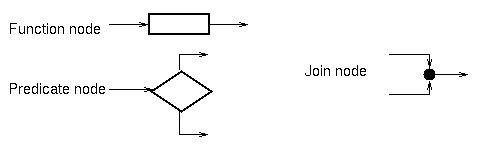
\includegraphics[width=\textwidth]{threeNodes}
\centering
\end{figure}

We define a \udef{proper program} as a flowchart which:
\begin{enumerate}
\item has a single entry arc;
\item has a single exit arc; and
\item has a path from the entry arc to each node and from each node to the exit arc.
\end{enumerate}

A \udef{prime program} is a proper program which has no embedded proper subprogram greater than one node. A sequence of function nodes is also considered prime.

A \udef{composite program} is a proper program that is not prime.

\begin{figure}[h]
\label{primeComposite}
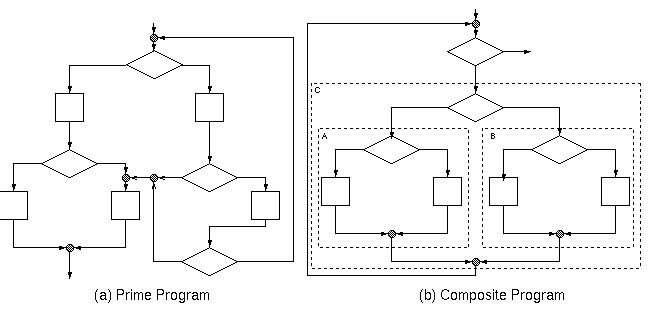
\includegraphics[width=\textwidth]{primeComposite}
\centering
\end{figure}

We can enumerate the prime programs. Figure \ref{primeEnumeration} describes all programs of up to $4$ nodes. 

\begin{figure}[h]
\label{primeEnumeration}
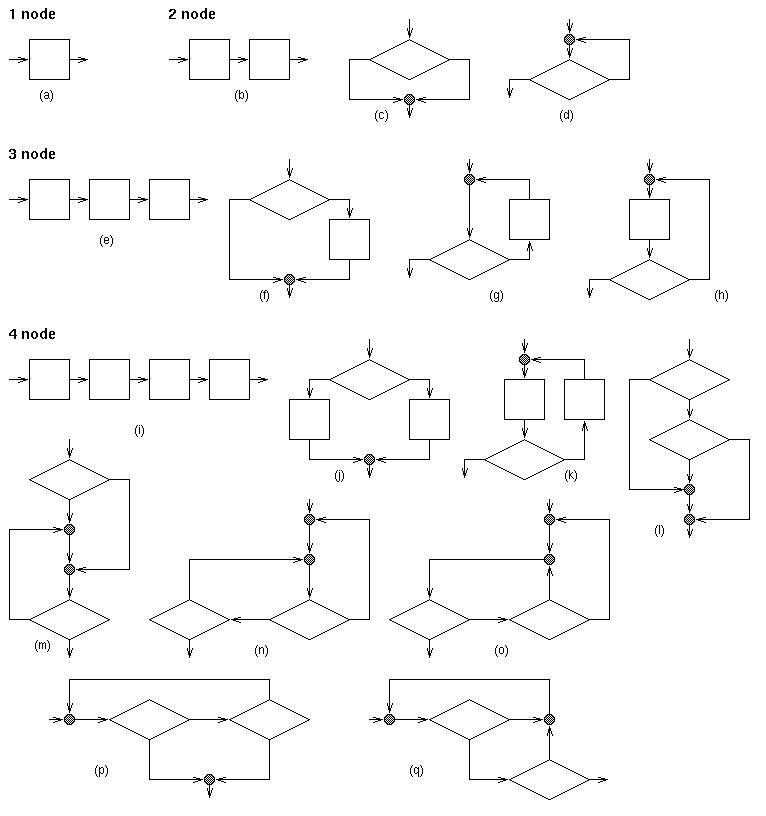
\includegraphics[width=\textwidth]{primeEnumeration}
\centering
\end{figure}

We can now classify these primes.
\begin{itemize}
\item Primes (a), (b), (e) and (i) represent sequences of function nodes.
\item Primes (c), (d), and (l) through (q) do not contain function nodes and thus do not change the state of the machine. They are either identity functions of or infinite loops.
\item The primes (f), (g), (h), (j) and (k) are the interesting primes. They represent the following control structures:
\item[(f)] is the \textbf{if-then},
\item[(g)] is the \textbf{while-loop},
\item[(h)] is the \textbf{do-while},
\item[(j)] is the \textbf{if-then-else} and
\item[(k)] is the \textbf{do-while-do}.
\end{itemize}
Most programming languages implement these control structures, except the do-while-do. This last structure has generally been ignored by language designers.

Other types of loops, such as for-loops can be considered syntactic sugar.
\subsubsection{Structured programming.}  
The goto statement is quite controversial. The paradigm of structured programming aims to improve clarity by eliminating goto statements and instead making use of the structured control flow constructs of selection (if/then/else) and repetition (while and for), block structures, and subroutines.

The goto statement has disadvantages:
\begin{enumerate}
\item The lack of hierarchical program structure can make programs less clear.
\item Making the order of statements in the program not necessarily the execution order can lead to confusion.
\item It violates the concept of \textit{one-in, one-out control structures}, making the design less understandable.
\item Groups of statements may serve multiple purposes. (On the other hand it can get rid of code duplication.)
\item It makes it hard to find a meaningful set of coordinates with which to describe the process progress. (See Dijkstra.)
\end{enumerate}


There are, however, also some advantages:
\begin{enumerate}
\item Direct hardware support. (This is relevant with poorly implemented Boolean variables and procedure calls, see in particular tail call optimization). TODO ref Knuth.
\item Simple and easy to use in small programs
\item Completely general purpose as a building block for simulating other control structures.
\item Some program structures are expressed more elegantly with a goto statement than with structures sequence control. Examples include:
\begin{itemize}
\item Loops with multiple natural exit points.
\item Simulating do-while-do loops.
\item Prematurely exiting a loop to deal with exceptional conditions.
\item When implementing state machines, state switches may conveniently be implemented using goto statements. This type of state-switching is often used in the Linux kernel.
\end{itemize}
In some languages these issues are addressed by using break statements, continue statements and throwing exceptions. All three of these however can be viewed as just a repackaging of the goto statement, with many of the same flaws.

Having said that, the practical consensus seems to be that these constructs are useful in practice.
\end{enumerate}

\subsubsection{Continuations}
First-class control
TODO?

\section{Subprogram control}
\subsection{Subprogram sequence control}
\subsubsection{Simple call-return.} In this view the main program may during execution call various subprograms, which may in turn call sub-subprograms. A very naive way to implement this is using the \textit{copy rule}: the code of the subprogram is simply copied into the main program whenever it is called.

Limitations of this naive view include the following:
\begin{enumerate}
\item \textit{Subprograms cannot be recursive.} A subprogram is \udef{directly recursive} if it calls itself at some point. A subprogram is \udef{indirectly recursive}	if it calls another subprogram that in turn calls the original subprogram.

If the copy rule were to be applied to a recursive subprogram, the resulting code would still call that subprogram. Thus we would be stuck in an infinite loop. This is problematic because recursion can be quite useful.

\item \textit{Subprograms must execute completely at each call.} Sometimes, however, we want the subprogram to resume execution from where it left off last time. This is essentially the idea behind coroutines.

\item \textit{Immediate transfer of control at point of call.} For a scheduled subprogram call we wish execution of the subprogram to be deferred until some later time.

\item \textit{Single execution sequence.} This implementation of subprograms does not support parallel programming.

\item \textit{Subprograms must be explicitly called.} Sometimes we do not know when we will want to call a subprogram. For instance an exception handler should be called whenever an exception is thrown. This is by definition exceptional.
\end{enumerate}

\paragraph{Implementation}
First we make a distinction between the \textit{definition} of a subprogram and its \textit{activation}. An activation record contains a reference to the code of the subprogram as well as an \textit{activation record} containing local data, parameters and other data.

Program flow is controlled by keeping track of pairs of pointers: The \udef{current-instruction pointer} (CIP) points to the statement currently being executed and the \udef{current-environment pointer} (CEP) points to the current activation record.

When a subprogram is called, the old CIP and CEP are stored somewhere. A new CIP is created pointing to the first statement of the code of the subprogram. A new CEP is created pointing to the newly created activation record.

When a subprogram ends, the old CIP and CEP are reinstated.

There are multiple ways the CIP and CEP may be stored. A stack may be used. Or they may be stored in the activation record of the new subprogram. If we only require the simple copy rule behaviour, we can even get away without the CEP: each subprogram can only ever have at most one activation record and thus we can statically allocate storage for a single activation record.

This simple model is often hardware-supported with a \textit{return-jump instruction}.

\subsubsection{Recursion.}
So long as both the CIP and CEP are stored, the implementation idea given above automatically supports recursion.

\subsubsection{Exceptions.} These are raised to signal exceptional circumstances, such as 
\begin{enumerate}
\item Error conditions
\item Unpredictable conditions
\item Tracing and monitoring
\end{enumerate}
An exception is typically propagated back up the call stack until the proper place th handle it.

The question of what to do once an exception has been handled does not have an obvious answer. Different languages have different solutions.
\paragraph{Assertions.} An assertion is a statement implying a relation among data in a program. During testing it will typically raise an error if that relation is violated. After testing it may remain as documentation. See also design by contract.

\subsubsection{Scheduling.} Scheduling can take several different forms, such as
\begin{enumerate}
\item Schedule subprograms to execute before or after other subprograms.
\item Schedule subprograms the be executed when a Boolean expression becomes true.
\item Schedule the execution of subprograms based on time.
\item Schedule subprograms based on priority.
\end{enumerate}

\subsubsection{Coroutines}. Coroutines are subprograms that can exit before completing execution. When it is called again, it resumes from where it left off. Two coroutines can pass control between themselves.

\subsubsection{Generators}. Generators, also known as semicoroutines, are like coroutines, but lack a coroutines ability to specify where it yields control to. It is still possible to implement coroutines on top of a generator facility, with the aid of a top-level dispatcher routine.

\subsubsection{Parallel programming}
TODO: move to separate section?
\paragraph{Things to take into account.} Parallel programming constructs add complexity to the language design. The following topics must be adressed.
\begin{enumerate}
\item \textit{Variable definitions.} If variables are mutable, we can run into synchronization problems. Definitional (i.e. immutable) variables do not have this problem.
\item \textit{Parallel composition.} We need ways to fork program execution and create additional threads of control.
\item \textit{Program structure}. Parallel programs generally follow one of two execution models:
\begin{enumerate}
\item They may be transformational, where the goal is to transform the input data into an appropriate output value. Parallelism is applied to speed up the process.
\item They may be reactive where the program reacts to external stimuli, called events.
\end{enumerate}
\item \textit{Communication} between parallel programs may happen through the use of shared memory or via messages.
\end{enumerate}
\paragraph{And or fork statements}
With this statement we can designate parts of the program that we can allow to be executed at the same time.

\paragraph{Guarded commands} These were proposed in the 1970s by Dijkstra. They provide a way to write nondeterministic programs.

A guarded statement has a condition, called a \udef{guard}, such that the statement is not executed if the guard is false. We consider the following types of guarded statements:
\begin{itemize}
\item The \textbf{guarded if statement} contains several guarded statements. At least one for the guards must be true. If multiple guards are true, the statement to execute is chosen nondeterministically.
\item The \textbf{guarded repetition statement} is like the guarded if statement that repeats as long as some guard is true.
\end{itemize}
TODO: move?? Also expand.

\paragraph{Tasks} Ordinarily when a subprogram is called, execution of the main program is suspended. If the subprogram is called as a task, the execution of the main program continues.

Task management can obviously be non trivial. In order for tasks running asynchronously to coordinate their activities, the language must provide some means of synchronization. This may be achieved in several ways:
\begin{enumerate}
\item \textbf{Interrupts}. If task A wishes to signal to task B that a particular event has occurred, then task A executes an instruction that causes the execution of task B to be interrupted immediately. Control is then handed to a subprogram or section of code that handles the interrupt. Afterwards control is handed back to task B.

This is a mechanism commonly found in computer hardware. It is also similar to exception handling. In high level-languages, interrupts have several disadvantages:
\begin{enumerate}
\item The code for interrupt handling is separate from the main body of the task, leading to a more confusing program structure.
\item A task waiting for an interrupt must usually enter a busy waiting loop.
\item The task must be written so that an interrupt can be handled at any time.
\end{enumerate}
\item \textbf{Semaphores}. TODO. A semaphore is a data object consisting of two parts:
\begin{enumerate}
\item An integer counter. In a binary semaphore this counter may only be one or zero, in a general semaphore it may be any non-negative integer.
\item A queue of tasks.
\end{enumerate}
Two operations are defined for a semaphore data object $P$:
\begin{enumerate}
\item \texttt{signal(P)}. When executed by a task A, this operation tests the value of the counter in $P$. If zero, the first task in the task queue is removed from the queue and executed. If not zero, or if the queue is empty, the counter is incremented by one. Execution of task A continues after the signal operation is complete.
\item \texttt{wait(P)}. When executed by task B, this operation tests the value of the counter in $P$. If nonzero, the counter is decremented by one and task B continues execution. If zero, task B is inserted at the end of the task queue for $P$ and the execution of B is suspended.
\end{enumerate}
Semaphores have some disadvantages for use in high-level languages:
\begin{enumerate}
\item A task can only wait for one semaphore at a time.
\item If a task fails to signal, the system of tasks may deadlock.
\item Programs with several tasks and semaphores become increasingly difficult to understand, debug and verify.
\item All tasks accessing the semaphore must share memory.
\end{enumerate}
\item \textbf{Messages} can be passed between tasks. The basic concept is similar to a pipe. Implementations of this system can be quite complex. Several tasks may simultaneously try to send messages. The implementation must then provide some way to store those messages until the receiver can process them.
\item \textbf{Guarded commands.} See above.
\item \textbf{Rendezvous.} Used in Ada. Like messages, but must be accepted.
\end{enumerate} 

\subsection{Shared data in subprograms}
Data can either be shared directly, using parameters, or indirectly by giving the subprogram access to nonlocal environments.

\subsubsection{Parameters and parameter transmission}
A \udef{(formal) parameter} is a variable declared in the function definition, that must be given some data when the function is called. This data that is given to the function is called an \udef{argument} or \udef{actual parameter}.

There are multiple ways to specify which argument should go to which parameter. This can, e.g., be done through positional correspondence or by explicitly naming the parameter.

There are also multiple ways to transmit parameters. Depending on the method of transmission, parameters can also be used to return data from the subprogram. In most languages a single value may also be returned as an explicit function value.

In some languages the distinction is made between between function calls with a return value and procedure or subroutine calls without a return value.

\paragraph{Call by name.} In this model the actual parameter is substituted everywhere for the formal parameter. This results in overhead leads to complications.
\paragraph{Call by reference.} A pointer to the location of the data object is made available to the subprogram.
\paragraph{Call by value.} The value of the argument is copied into a variable with the name of the formal parameter.
\paragraph{Call by value-result.} Like call by value, except at the end of the subprogram the contents of the local variable is copied back into the original argument variable.
\paragraph{Call by constant value.} The formal argument acts like a local constant.
\paragraph{Call by result.} This parameter is only used to transmit a result back from a subprogram. 

\subsubsection{Data sharing through environments.}
TODO
\paragraph{Explicit common environments.}
TODO

\subsection{First-class subprograms}
If we say a language has first-class subprograms or functions, it means functions are treated just like any other data type. TODO

\subsubsection{Closures}
TODO

\subsection{Factors that obscure the definition of subprograms as mathematical functions}
\begin{enumerate}
\item Implicit arguments.
\item Implicit results (side-effects).
\item Behaviour can be undefined for some arguments. In general the domain is too broad and needs to be narrowed with conditional statements.
\item History sensitive.
\end{enumerate}

\subsection{Tail call optimization}
TODO


\section{Miscellaneous language features}
TODO Reflection


\section{Tools}
\subsection{ANTLR}
\subsection{YACC - LEX / BISON}
\subsection{LLVM}
Also JVM, GCC?
\subsection{Racket}
